\section{Números primos}
	\subsection{Descripción del problema}
	Desarrollar un programa que encuentre todos los números primos en el intervalo $0 \leq n \leq 1000$ imprimirlos en pantalla junto con su representación en binario ademas de contar la cantidad de ceros y unos en dicho numero, finalmente guarda los números primos en su forma binaria en un archivo txt.
	Cuenta con modo manual (el usuario ingresa un numero n) y automático (el programa utiliza un $n$ aleatorio).
	\subsection{Código}
	El código del programa fue realizado en Python 3.5.
	\\
	Archivo: primos.py
		\begin{lstlisting}[language=Python]
		# primos.py
		# -*- coding: utf-8 -*-
		from __future__ import print_function
		import math, random
		
		separador = '*'*50
		
		def iniciar():
		maximo = 1
		continuar = True
		
		while continuar:
			archivo = open('primos.txt', 'w')
			lista_primos = []
			lista_binarios = []
			manual = imprimir_menu()
			if manual == 1:
				maximo = int(input("Escribe un numero entre 1 y 1000 "))
			elif manual == 2:
				maximo = random_maximo()
			else:
				break
			print("El limite es: ", maximo)
			lista_primos = calcular_primos(maximo)
			lista_binarios = conversion_binaria(lista_primos, archivo)
			print(lista_primos)
			print('*'*50)
			print(lista_binarios)
			contar_repeticiones(lista_binarios, lista_primos)
			print('Numeros primos en binarios guardados en primos.txt')
			archivo.close()
			opcion = input("Reintentar s/n: ")
			if opcion.lower() != 's':
				continuar = False
			
		print('Saliendo...')
		
		def random_maximo():
			return random.randint(1, 1000)
		
		def calcular_primos(maximo):
			lista_primos = []
			es_primo = False
			if maximo < 2:
				es_primo = False
			else:
				lista_primos.append(2)
				for numero_actual in range(2, maximo + 1):
					raiz = math.sqrt(numero_actual)
					if raiz == round(raiz):
						es_primo = False
					else:
						for num in lista_primos:
							if num > math.ceil(raiz):
								break
							if numero_actual % num == 0:
								es_primo = False
								break
							else:
								es_primo = True
						if es_primo:
							lista_primos.append(numero_actual)
			return lista_primos
		
		def imprimir_menu():
			print('\n\n%sMenu%s' % (separador, separador))
			print("""
			1.- Manual
			2.- Automatico
			3.- Salir
			""")
			try:
				opcion = int(input("Selecciona una opcion valida: "))
				return opcion
			except Exception as e:
				print('Error ', e)
				return 0
		
		def conversion_binaria(lista_primos, archivo):
			lista_binarios = []
			archivo.write('{')
			for numero in lista_primos:
				lista_binarios.append(bin(numero)[2:])
				archivo.write('%s,' % bin(numero)[2:])
			
			archivo.write('}')
			return lista_binarios
		
		def contar_repeticiones(lista_binarios, lista_primos):
			total = []
			i = 0
			for valor in lista_binarios:
				ceros, unos = 0, 0
				for digito in valor:
					if digito == '0':
						ceros += 1
					else:
						unos += 1
				total.append({'Numero': lista_primos[i], 'Ceros': ceros, 'Unos': unos})
				i += 1
			for numero in total:
				print('Numero: %s No. Ceros: %s No. Unos: %s' % (numero['Numero'], numero['Ceros'], numero['Unos']))
			
		iniciar()
		
		\end{lstlisting}
	\subsection{Pruebas}
	Las pruebas están divididas en modo automático y manual.
	\\{\large Modo automático.}
		\begin{figure}[H]
			\begin{center}
				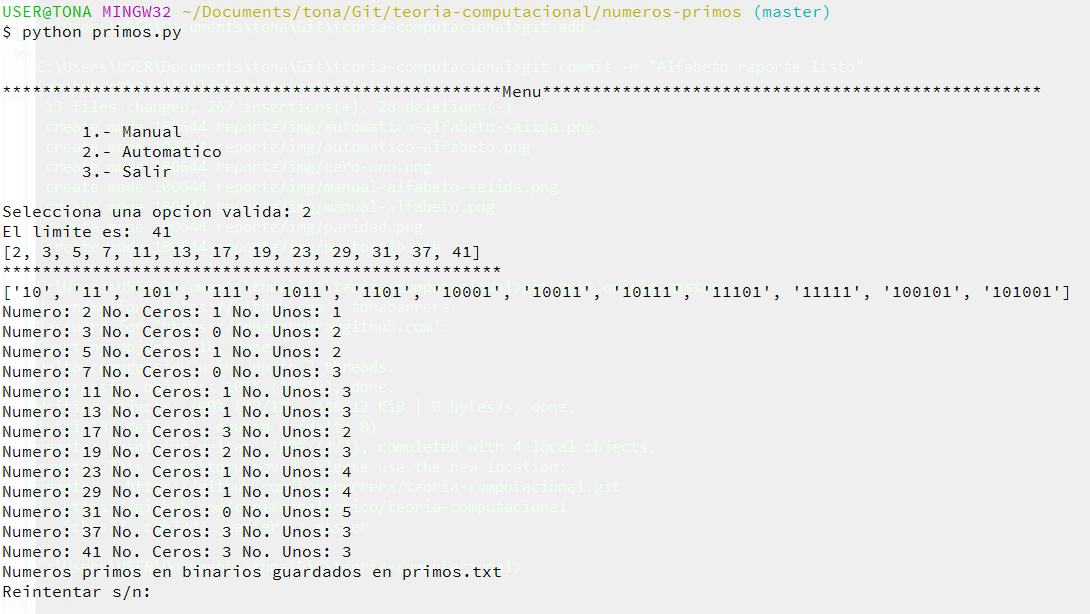
\includegraphics[width=\linewidth, height=6cm]{img/primos-automatico.png}
				\caption{Modo automático n=41.}
				\label{fig:primos1}
			\end{center}
		\end{figure}
			\begin{figure}[H]
				\begin{center}
					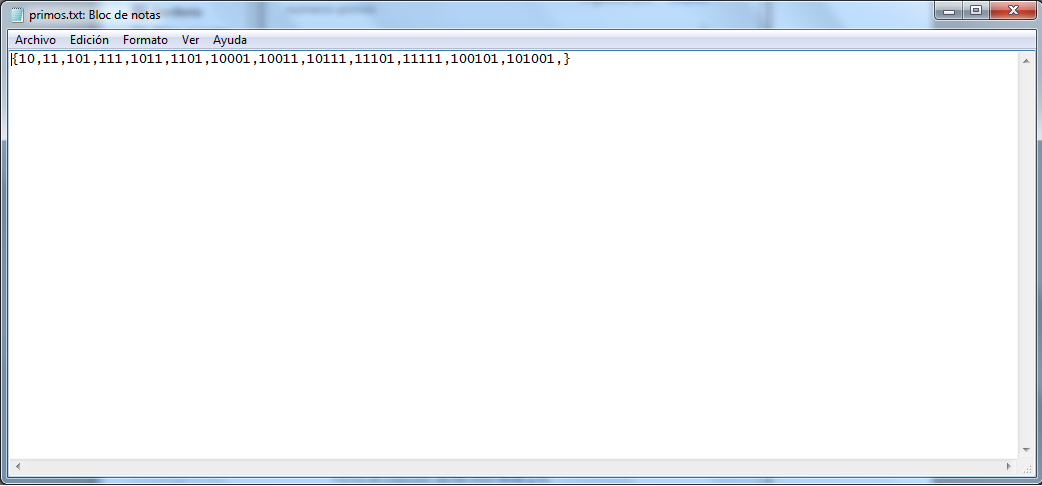
\includegraphics[width=\linewidth, height=7cm]{img/primos-automatico-salida.png}
					\caption{Números primos en binario en el archivo.}
					\label{fig:primos2}
				\end{center}
			\end{figure}
	{\large Modo manual.}
		\begin{figure}[H]
			\begin{center}
				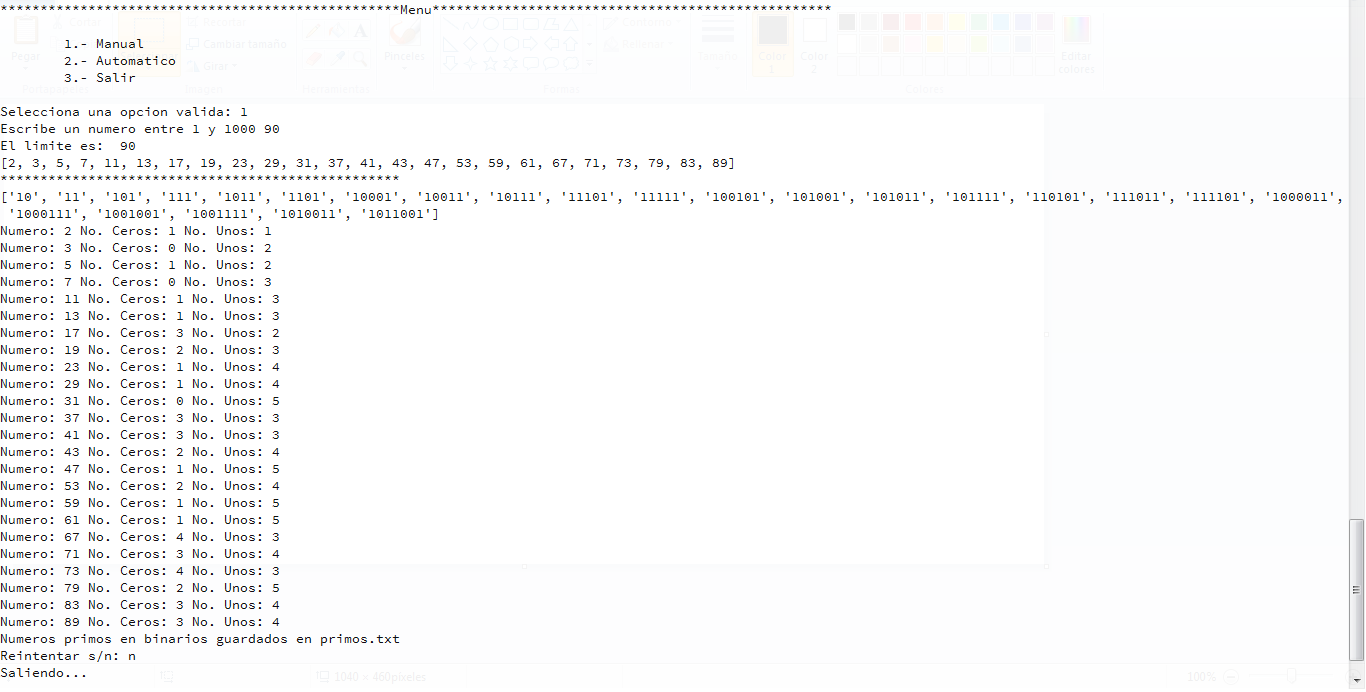
\includegraphics[width=\linewidth, height=10cm]{img/primos-manual.png}
				\caption{Modo automático n=90.}
				\label{fig:primos3}
			\end{center}
		\end{figure}
			\begin{figure}[H]
				\begin{center}
					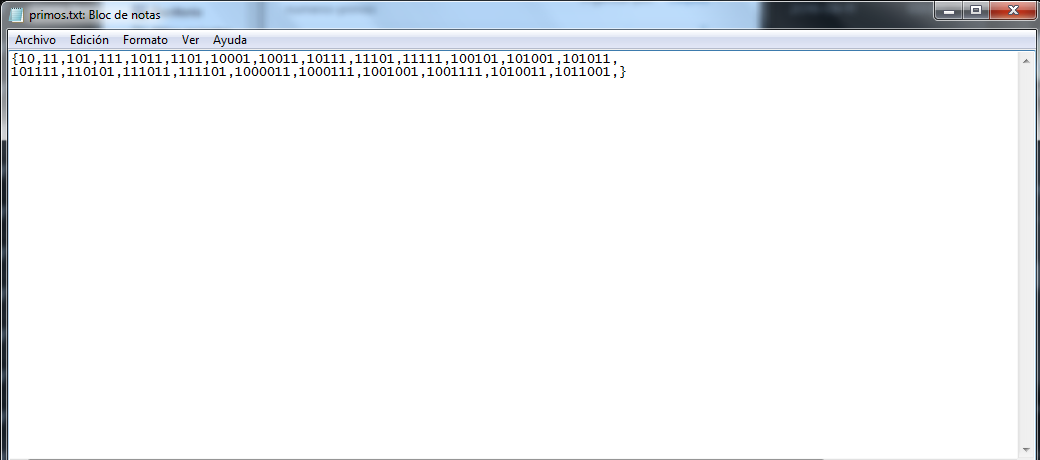
\includegraphics[width=\linewidth, height=7cm]{img/primos-manual-salida.png}
					\caption{Números primos en binario en el archivo.}
					\label{fig:primos4}
				\end{center}
			\end{figure}
	\begin{figure}[H]
		\begin{center}
			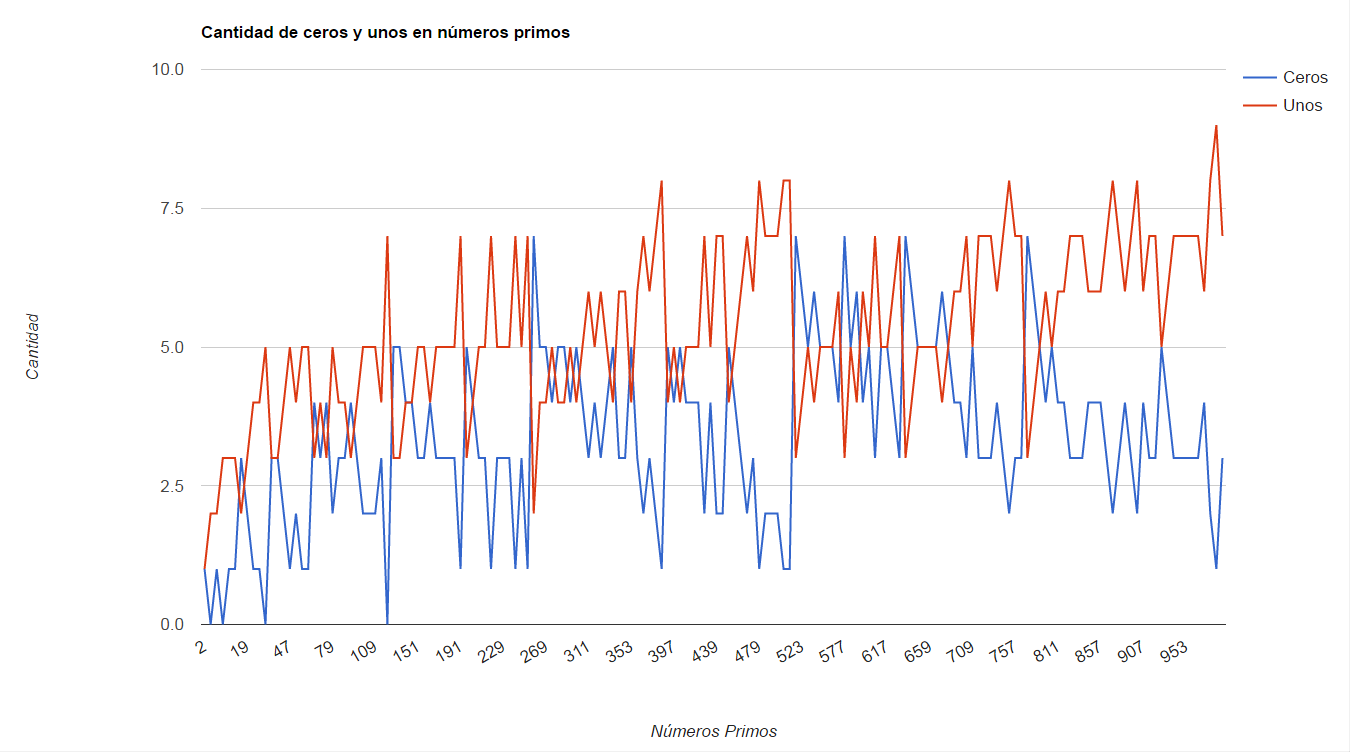
\includegraphics[width=\linewidth, height=7cm]{img/primos.png}
			\caption{Cantidad de ceros y unos encontrados entre 1 y 1000.}
			\label{fig:grafica}
		\end{center}
	\end{figure}